\documentclass{beamer}
\usepackage[T1]{fontenc}
\usepackage[utf8]{inputenc}
\usepackage{lmodern}
\usepackage[brazil]{babel}
\usepackage{color}

\usetheme{JuanLesPins}

\title{Frete Fácil}
\author{Caio Teixeira da Quinta\\
        Giancarlo Rigo\\
        Rafael Reggiani Manzo\\
        Willen Goulart}

\begin{document}

\maketitle

\section{Introdução}
\begin{frame}
  \frametitle{Frete Fácil}
  \framesubtitle{Empresa}

  A Frete Fácil é uma empresa de intermediação de serviços de frete, que combina a necessidade de um cliente por um frete em um período de tempo, local e por um valor máximo, com a vontade de um transportador de aumentar seus rendimentos e reduzir a ociosidade de sua frota.  
\end{frame}

\begin{frame}
  \frametitle{Produto}
  \framesubtitle{}

  Plataforma de intermediação de serviços de frete, na qual:
    \begin{itemize}
    \item O cliente informa locais de origem e destino, dimensões, tempo e preço máximo;
    \item Com base nessas informações, a plataforma encontra transportadores para realizar o frete;
    \item Após os transportadores aceitarem o frete, o cliente escolhe o transportador através das opnião de outros usuários;
    \item Os dados para contato são apresentados tanto para o cliente quanto ao transportador;
    \item Os valores para cobrança são calculados.
    \end{itemize}
\end{frame}

\begin{frame}
  \frametitle{Motivação}
  \framesubtitle{}
  
  Motivações para os clientes:
    \begin{itemize}
    \item Dificuldade em encontrar fretes baratos;
    \item Dificuldade de encontrar avaliações sobre transportadores;
    \item Dificuldade de transportar cargas fragéis, como instrumentos musicais, animais e plantas.
    \end{itemize}
\end{frame}

\begin{frame}
  \frametitle{Motivação}
  \framesubtitle{}
  
  Motivações para os transportadores:
    \begin{itemize}
    \item Fracionamento de cargas;
    \item Frete de volta;
      \begin{itemize}
      \item Frete de volta costumam ter o valor 50\% menor do que o frete de ida;\\
      \item Para conseguir um frete de volta é necessário conhecer o mercado da região ou fazê-lo através de outra transportadora que retém de 30\% a 40\% do valor do frete.
      \end{itemize}
    \end{itemize}
\end{frame}


\section{Análise de mercado}

\begin{frame}
  \frametitle{Análise de mercado}
  \framesubtitle{}

  \begin{center}
    {\huge\textbf{Análise de Mercado}}

  \end{center}
\end{frame}

\begin{frame}
  \frametitle{Mercado atual}

  \framesubtitle{Perfil dos Clientes}
      \begin{itemize}
      \item Serviço focado em micro e pequenas empresas transportadoras além de profissionais autônomos e cooperativas de transporte.
      \end{itemize}
\end{frame}

\begin{frame}
  \frametitle{Mercado atual}
  \framesubtitle{Mercado Potencial}
      \begin{itemize}
      \item Existem cerca de 62.789 empresas de transporte de cargas e apenas 4679 com 20 ou mais empregados (Fonte: IBGE)
      \item A participação de microempresas no setor corresponde a 92\% do total enquanto as pequenas-empresas(10 a 49 empregados) correspondem à 7\%(Fonte: IBGE).
      \item Segunto a ANTT existem cerca 680 cooperativas de carga compostas por autônomos.
      \end{itemize}
\end{frame}
\section{Plano de marketing}

\begin{frame}
  \frametitle{}
  \framesubtitle{}

  \begin{center}
    {\huge\textbf{Plano de Marketing}}
  \end{center}
\end{frame}

\begin{frame}
  \frametitle{Produtos}
  \framesubtitle{}

\end{frame}

\begin{frame}
  \frametitle{Precificação}
  \framesubtitle{}

\end{frame}

\begin{frame}
  \frametitle{Estratégias promocionais}
  \framesubtitle{}

\end{frame}

\begin{frame}
  \frametitle{Estrutura de comercialização}
  \framesubtitle{}

\end{frame}

\section{Plano operacional}
\begin{frame}
  \frametitle{}
  \framesubtitle{}

  \begin{center}
    {\huge\textbf{Plano Operacional}}
  \end{center}
\end{frame}

\begin{frame}
  \frametitle{Capacidade produtiva}
  \framesubtitle{Novas funcionalidades e atendimento a clientes}

  \begin{itemize}
    \item 160 horas de trabalho semanais no desenvolvimento do produto;
    \item Capacidade para até 175 empresas por mês;
    \item E intermediar até 1575 fretes por mês;
  \end{itemize}

\end{frame}

\begin{frame}
  \frametitle{Processos operacionais}
  \framesubtitle{}

  Estão previstos os processos básico da vida da empresa:
  \begin{itemize}
    \item Ciclo de desenvolvimento;
    \item Processo de aquisição de infraestrutura computacional;
    \item Divulgação da plataforma;
    \item Suporte a clientes.
  \end{itemize}

\end{frame}

\begin{frame}
  \frametitle{Pessoal}

  Será contratada uma pessoa para se dedicar a dar suporte aos clientes.

\end{frame}

\section{Plano Financeiro}
\begin{frame}
  \frametitle{}
  \framesubtitle{}

  \begin{center}
    {\huge\textbf{Plano Financeiro}}
  \end{center}
\end{frame}

\begin{frame}
  \frametitle{Demonstrativo de resultados}
  \framesubtitle{Evolução no tempo}

  \begin{center}
    \frame{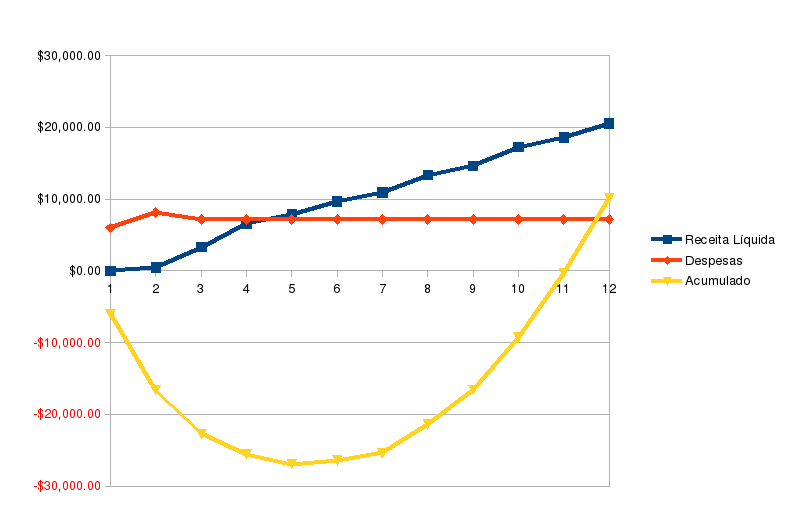
\includegraphics[width=100mm, height=60mm]{images/evolucao-financeira.png}}
  \end{center}
\end{frame}

\begin{frame}
  \frametitle{Demonstrativo de resultados}
  \framesubtitle{Expectativa para o primeiro ano}

  \begin{small}
    \begin{tabular}{| l | l |}
      \hline
      \textbf{Descrição} & \textbf{Valor (R\$)}\\ \hline
      1. Receita total com vendas & \textcolor{green}{130.350,00}\\ \hline \hline
      2. Custos variáveis totais & \textcolor{red}{113.605,68}\\ \hline
      (-) Custo das mercadorias vendidas & \textcolor{red}{9.871,00}\\ \hline
      (-) Impostos sobre vendas & \textcolor{red}{7.734,68} \\ \hline
      (-) Custos com mão-de-obra & \textcolor{red}{96.000,00} (8.000 X 12)\\ \hline \hline
      3. Margem de contribuição (1 - 2) & \textcolor{green}{16.764,32}\\ \hline \hline
      4. (-) Custos fixos totais & \textcolor{red}{15.120,00} (1.260 X 12)\\ \hline \hline
      5. Resultado Operacional (Lucro/Prejuízo) (3 – 4) & \textcolor{green}{1.624,32}\\ \hline
    \end{tabular}
  \end{small}
\end{frame}

\begin{frame}
  \frametitle{Indicadores de viabilidade}
  \framesubtitle{Ponto de equilíbrio}

  \begin{tabular}{| l | l |}
    \hline
    \textbf{Receita total:} & R\$ 130.350,00 \\ \hline
    \textbf{Custo variável total:} & R\$ 113.605,68 \\ \hline
    \textbf{Custo fixo total:} & 15.120,00 \\ \hline
  \end{tabular}

  \begin{itemize}
    \item \textbf{Índice da margem de contribuição:} $\frac{130350 - 113605,68}{130350} \cong 0.13$
    \item \textbf{Ponto de equilíbrio:} $\frac{15120}{0.13} = 116307,69$
  \end{itemize}

  Portanto, a empresa estará cobrindo seus custos a partir do momento em que atingir uma receita bruta total de R\$ 116.307,69.
\end{frame}

\begin{frame}
  \frametitle{Indicadores de viabilidade}
  \framesubtitle{Lucratividade}

  \begin{tabular}{| l | l |}
    \hline
    \textbf{Receita total:} & R\$ 130.350,00 \\ \hline
    \textbf{Lucro líquido:} & R\$ 10.753,75 \\ \hline
  \end{tabular}

  .\newline \newline

  Resultando em uma lucratividade de $\frac{10753,75}{130350} \cong 8\%$.
\end{frame}

\begin{frame}
  \frametitle{Indicadores de viabilidade}
  \framesubtitle{Rentabilidade e prazo de retorno}

  \begin{tabular}{| l | l |}
    \hline
    \textbf{Lucro líquido:} & R\$ 10.753,75 \\ \hline
    \textbf{Investimento total:} & R\$ 10.392,00 \\ \hline
  \end{tabular}

  .\newline \newline

  \begin{itemize}
    \item Resultando em uma lucratividade de $\frac{10753,75}{10392}*100 \cong 103\%$ ao ano.
    \item Desta forma recuperando o investimento antes do primeiro ano.
  \end{itemize}
\end{frame}

\section{Construção de cenários}
\begin{frame}
  \frametitle{}
  \framesubtitle{}

  \begin{center}
    {\huge\textbf{Construção de Cenários}}
  \end{center}
\end{frame}

\section{Avaliação estratégica}
\begin{frame}
  \frametitle{}
  \framesubtitle{}

  \begin{center}
    {\huge\textbf{Avaliação Estratégica}}
  \end{center}
\end{frame}

\begin{frame}
  \frametitle{Avaliação Estratégica}
  \framesubtitle{Matriz SWOT}
  \begin{tabular}{|p{5.0cm}|p{5.0cm}|}
  \hline
   \textbf{Forças} & \textbf{Fraquezas}\\ \hline
    Competência Técnica & Pouco Know-How do Meio \\ \hline
   Facilidade de Implementação & Capital Inicial Restrito \\ \hline
   Investimento Inicial Baixo & Adesão das Transportadoras\\ \hline
   Sem necessidade de lidar com transações financeiras diretamente &  Falta de designers e marketeiros dentre os integrantes \\ \hline
    \textbf{Oportunidades} & \textbf{Ameaças}\\ \hline
Sem serviços semelhantes no mercado & Possível Competição com grandes transportadoras\\ \hline
Transporte rodoviário é a pricipal  forma de transportar cargas no país & Garantir a confiabilidade do Sistema \\   \hline
   Preço final acessível para o Cliente & Pouca divulgação do Sistema\\ \hline
  \end{tabular}
\end{frame}
\end{document}
